\documentclass{article}
\usepackage{fullpage}
\usepackage{tikz}
\usepackage{tkz-graph}
\usepackage[dvipsnames]{xcolor}
\usetikzlibrary{arrows.meta, positioning, shadows, shapes.geometric, fit, backgrounds, shapes.misc}
%\documentclass[tikz,border=10pt]{standalone}
% \usetikzlibrary{shapes.geometric, arrows.meta, positioning}
\usepackage{caption}


\def\AlonzoColor{Periwinkle}
\def\BabbageColor{Tan}
\def\ConwayColor{yellow!50}
\def\ShelleyColor{lightgray}

\newcommand{\legendbox}[1]{%
  \textcolor{#1}{\rule{\fontcharht\font`X}{\fontcharht\font`X}}%
}
\begin{document}

\begin{figure}
  \centering

    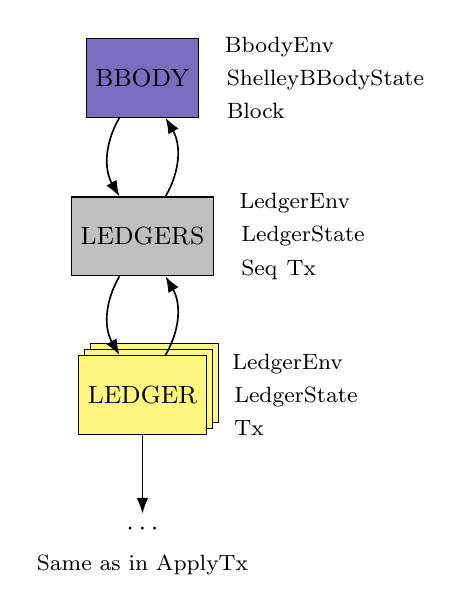
\begin{tikzpicture}[
% node distance = 4mm and 8mm,
     N/.style = {draw, fill=white, minimum size=1cm, align=right},
   dcs/.style = {double copy shadow, shadow xshift=2pt, shadow yshift=-2pt},
    every edge/.style={draw, ->, >=Latex,semithick}
%every edge/.append style = {draw, semithick, -Stealth}
                        ]
\node[N, fill=\AlonzoColor
     , label={[text width=26mm]east: {\footnotesize \phantom{i} BbodyEnv \phantom{X}ShelleyBBodyState \phantom{X}Block}}
     ] (bbody)  {\small BBODY};
\node[N, below =of bbody, fill=\ShelleyColor
     , label={[text width=20mm]east: {\footnotesize \phantom{i} LedgerEnv \phantom{X}LedgerState \phantom{X}Seq Tx}}
     ]  (ledgers)       {\small LEDGERS};
\node[N
     , label={[text width=20mm]east: {\footnotesize \phantom{i} LedgerEnv \phantom{X}LedgerState \phantom{X}Tx}}
     , below =of ledgers, dcs, fill=\ConwayColor
     ]  (ledger)       {\small LEDGER};
\node[label={south: {\footnotesize Same as in ApplyTx}}
     , below =of ledger]  (dots)       {$\cdots$};

\draw   (bbody)   edge[bend right] (ledgers)
        (ledgers) edge[bend right] (bbody)
        (ledgers) edge[bend right] (ledger)
        (ledger)  edge[bend right] (ledgers)
        (ledger)  edge (dots);
    \end{tikzpicture}

\caption{ApplyBlock.applyBlockOpts module (\legendbox{\AlonzoColor}~Alonzo, \legendbox{\ShelleyColor}~Shelley, \legendbox{\ConwayColor}~Conway)}
\label{fig:apply-block}
\end{figure}


\begin{figure}
  \centering
  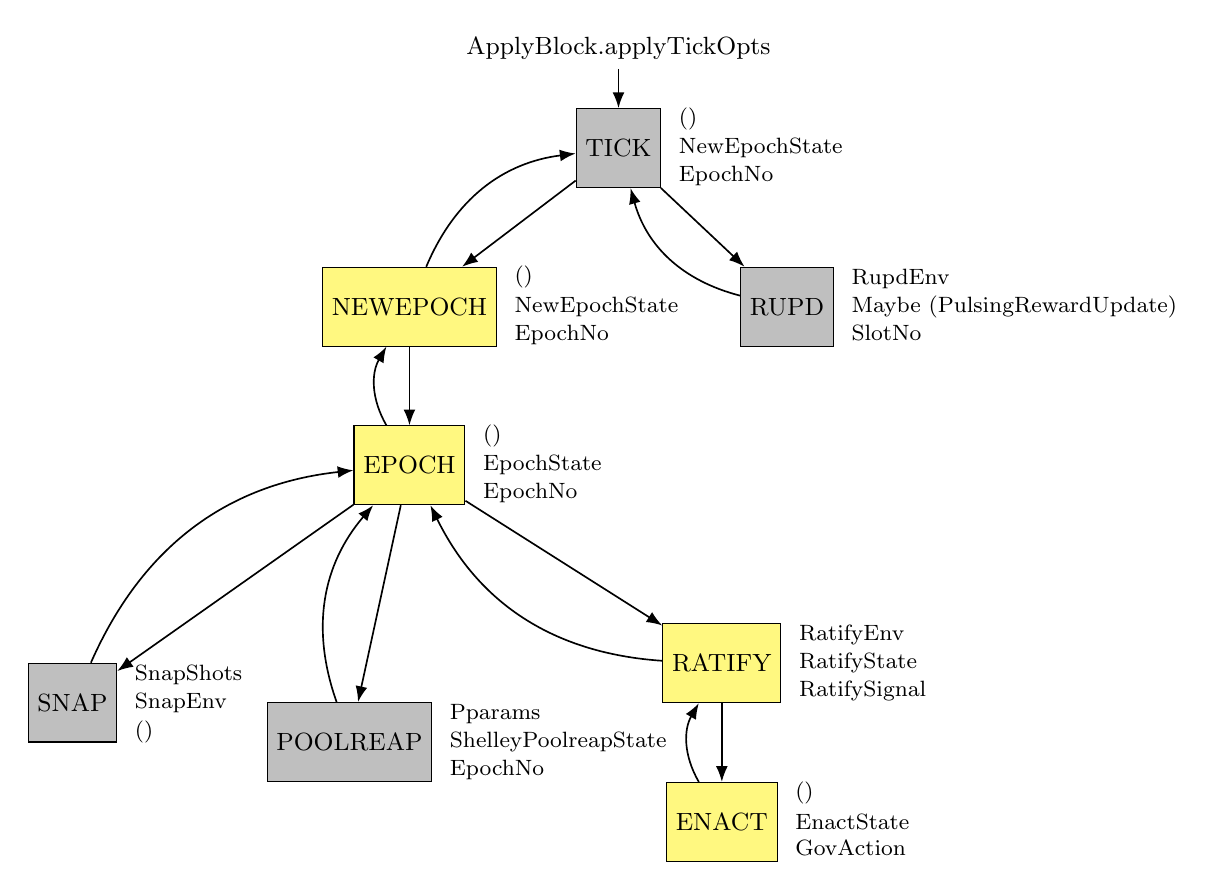
\begin{tikzpicture} [
    N/.style = {draw, fill=white, minimum size=1cm, align=right},
    dcs/.style = {double copy shadow, shadow xshift=2pt, shadow yshift=-2pt},
    every edge/.style={draw, ->, >=Latex,semithick}
    ]

  %%% TICK %%%
  \node[ N, fill=\ShelleyColor] (tick) {\small TICK};
    % text labels
    \node  [above right =-4mm and 1mm of tick] {\footnotesize ()};
    \node  [right =1mm of tick] {\footnotesize NewEpochState};
    \node  [below right =-4mm and 1mm of tick] {\footnotesize EpochNo};

  %%% ApplyBlock (TOP) %%%
  \node (applyblock) [above =5mm of tick] {\small ApplyBlock.applyTickOpts};

  %%% NEWEPOCH %%%
  \node[N,fill=\ConwayColor] (newepoch) [below left = of tick]   {\small NEWEPOCH}; % {\textcolor{white}
    % text labels
    \node  [above right =-4mm and 1mm of newepoch] {\footnotesize ()};
    \node  [right =1mm of newepoch] {\footnotesize NewEpochState};
    \node  [below right =-4mm and 1mm of newepoch] {\footnotesize EpochNo};

  %%% RUPD %%%
  \node[N,fill=\ShelleyColor] (rupd)     [below right =1cm and 1cm of tick]  {\small RUPD};
    % text labels
    \node  [above right =-4mm and 1mm of rupd] {\footnotesize RupdEnv};
    \node  [right =1mm of rupd] {\footnotesize Maybe (PulsingRewardUpdate)};
    \node  [below right =-4mm and 1mm of rupd] {\footnotesize SlotNo};

  %%% EPOCH %%%
  \node[N,fill=\ConwayColor] (epoch)    [below = of newepoch]    {\small EPOCH};
    % text labels
    \node  [above right =-4mm and 1mm of epoch] {\footnotesize ()};
    \node  [right =1mm of epoch] {\footnotesize EpochState};
    \node  [below right =-4mm and 1mm of epoch] {\footnotesize EpochNo};

  %%% SNAP %%%
  \node[N,fill=\ShelleyColor] (snap)     [below left = 2cm and 3cm of epoch]  {\small SNAP};
    % text labels
    \node  [above right =-4mm and 1mm of snap] {\footnotesize SnapShots};
    \node  [right =1mm of snap] {\footnotesize SnapEnv};
    \node  [below right =-4mm and 1mm of snap] {\footnotesize ()};

  %%% POOLREAP %%%
  \node[N,fill=\ShelleyColor] (poolreap) [below left = 25mm and -1cm of epoch]       {\small POOLREAP};
    % text labels
    \node  [above right =-4mm and 1mm of poolreap] {\footnotesize Pparams};
    \node  [right =1mm of poolreap] {\footnotesize ShelleyPoolreapState};
    \node  [below right =-4mm and 1mm of poolreap] {\footnotesize EpochNo};

  %%% RATIFY %%%
  \node[N,fill=\ConwayColor] (ratify)   [below right = 15mm and 25mm of epoch] {\small RATIFY};
    % text labels
    \node  [above right =-4mm and 1mm of ratify] {\footnotesize RatifyEnv};
    \node  [right =1mm of ratify] {\footnotesize RatifyState};
    \node  [below right =-4mm and 1mm of ratify] {\footnotesize RatifySignal};

  %%% ENACT %%%
  \node[N,fill=\ConwayColor] (enact)    [below = of ratify]      {\small ENACT};
    % text labels
    \node  [above right =-4mm and 1mm of enact] {\footnotesize ()};
    \node  [right =1mm of enact] {\footnotesize EnactState};
    \node  [below right =-4mm and 1mm of enact] {\footnotesize GovAction};

  % Edges
  \path (tick) edge (newepoch);
  \path (tick) edge (rupd);

  \path (applyblock) edge (tick);

  \path (newepoch) edge[bend left] (tick);
  \path (newepoch) edge (epoch);

  \path (rupd) edge[bend left] (tick);

  \path (epoch) edge[bend left] (newepoch);
  \path (epoch) edge (snap);
  \path (epoch) edge (poolreap);
  \path (epoch) edge (ratify);

  \path (snap) edge[bend left] (epoch);
  \path (poolreap) edge[bend left] (epoch);
  \path (ratify) edge[bend left] (epoch);

  \path (ratify) edge (enact);
  \path (enact) edge[bend left] (ratify);


  \end{tikzpicture}
\caption{API.Validation module (\legendbox{\ShelleyColor}~Shelley, \legendbox{\ConwayColor}~Conway)}
\label{fig:api-validation-diagram}
\end{figure}




\begin{figure}
  \centering
  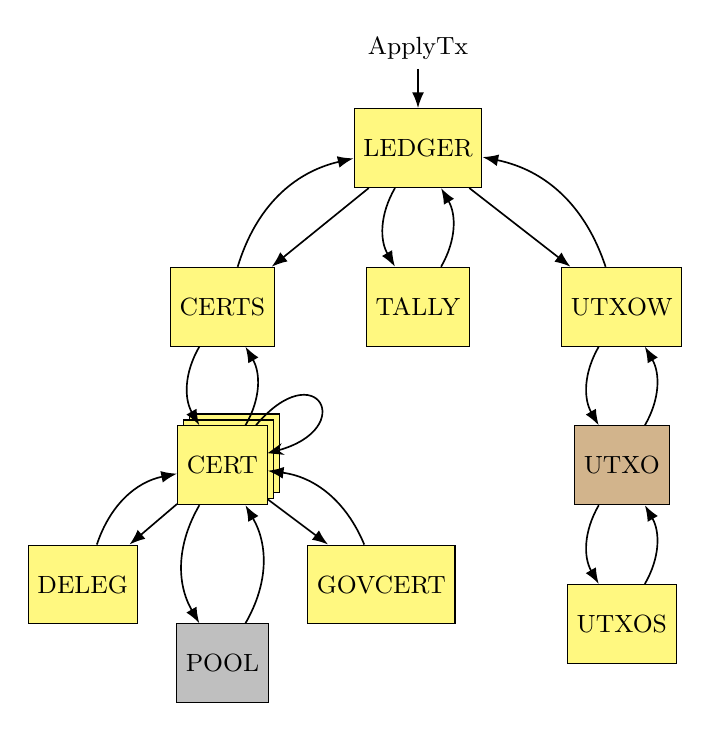
\begin{tikzpicture} [
     N/.style = {draw, fill=white, minimum size=1cm, align=right},
   dcs/.style = {double copy shadow, shadow xshift=2pt, shadow yshift=-2pt},
    every edge/.style={draw, ->, >=Latex,semithick}
% every edge/.append style = {draw, semithick, -Stealth}
]
% every node/.style={draw, shape=ellipse, minimum size=6mm, inner sep=2pt},
%     every edge/.style={draw, ->, >=Latex},
%     dotted edge/.style={draw, ->, >=Latex, dotted}
    % , level distance=2cm
    % , sibling distance=3cm
  % ]

  % Nodes and Positions
  % LEVEL 0 (TOP)
  \node[N, fill=\ConwayColor] (ledger) {\small LEDGER};
  \node (applytx) [above =5mm of ledger] {\small ApplyTx};

  % LEVEL -1
  \node[N, fill=\ConwayColor] (certs) [below left =of ledger] {\small CERTS};
  \node[N, fill=\ConwayColor] (tally) [below      =of ledger] {\small TALLY};
  \node[N, fill=\ConwayColor] (utxow) [below right=of ledger] {\small UTXOW};

  % \node (certs) [below left=1cm and -2mm of CHAIN] {\small CERTS};
  % \node (tally) [below right=1cm and 0mm of CHAIN] {\small TALLY};
  % \node (utxow) [below right=1cm and 0mm of CHAIN] {\small UTXOW};

  % LEVEL -2
  \node[N, fill=\ConwayColor, dcs] (cert) [below =of certs] {\small CERT};
  \node[N, fill=\BabbageColor] (utxo) [below =of utxow] {\small UTXO};

  % LEVEL -3 %1cm and 0mm
  \node[N, fill=\ConwayColor]  (deleg)   [below left =5mm and 5mm of cert] {\small DELEG};
  \node[N, fill=\ShelleyColor] (pool)    [below      =15mm of cert] {\small POOL};
  \node[N, fill=\ConwayColor]  (govcert) [below right=5mm and 5mm of cert] {\small GOVCERT};
  \node[N, fill=\ConwayColor]  (utxos)    [below =of utxo]                 {\small UTXOS};

  % Edges
  \path (applytx) edge (ledger);
  \path (ledger) edge (certs);
  \path (ledger) edge[bend right] (tally);
  \path (ledger) edge (utxow);

  \path (certs) edge[bend left] (ledger);
  \path (tally) edge[bend right] (ledger);
  \path (utxow) edge[bend right] (ledger);

  \path (certs) edge[bend right] (cert);
  \path (cert) edge[bend right] (certs);

  % \path[->,every loop/.style={looseness=5}] (cert) edge [loop right] ();
  % \Loop[dist=15mm,dir=NOEA](cert)
  \draw[semithick,->, -Stealth] (cert) to [looseness=8, out=50,in=15] (cert);

  \path (cert) edge (deleg);
  \path (cert) edge [bend right] (pool);
  \path (cert) edge (govcert);

  \path (deleg)   edge [bend left]  (cert);
  \path (pool)    edge [bend right] (cert);
  \path (govcert) edge [bend right] (cert);

  \path (utxow) edge [bend right] (utxo);
  \path (utxo) edge [bend right] (utxow);

  \path (utxo) edge [bend right] (utxos);
  \path (utxos) edge [bend right] (utxo);

  \end{tikzpicture}
\caption{API.MemPool module (\legendbox{\ShelleyColor}~Shelley, \legendbox{\ConwayColor}~Conway, \legendbox{\BabbageColor}~Babbage)}
\label{fig:api-mempool}
\end{figure}



\begin{figure}
  \centering
  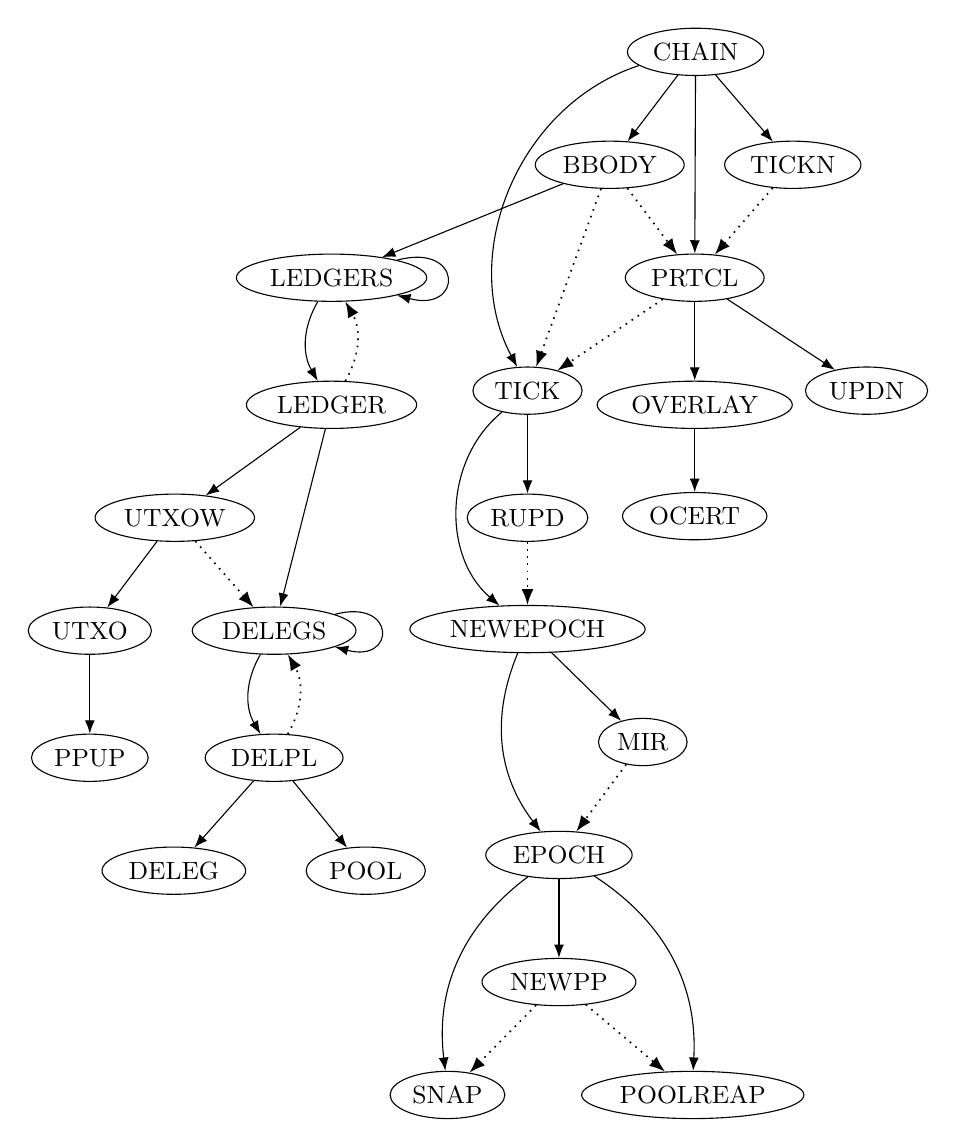
\begin{tikzpicture} [
    every node/.style={draw, shape=ellipse, minimum size=6mm, inner sep=2pt},
    every edge/.style={draw, ->, >=Latex},
    dotted edge/.style={draw, ->, >=Latex, dotted, semithick}
    % , level distance=2cm
    % , sibling distance=3cm
  ]

  % Nodes and Positions
  % LEVEL 0 (TOP)
  \node (CHAIN) {\small CHAIN};

  % LEVEL -1
  \node (BBODY) [below left=1cm and -2mm of CHAIN] {\small BBODY};
  \node (TICKN) [below right=1cm and 0mm of CHAIN] {\small TICKN};

  % LEVEL -2
  \node (LEDGERS) [below left=1cm and 2cm of BBODY] {\small LEDGERS};
  \node (PRTCL) [below left=1cm and 0mm of TICKN] {\small PRTCL};

  % LEVEL -3
  \node (LEDGER) [below=of LEDGERS] {\small LEDGER};
  \node (TICK) [below left=of PRTCL] {\small TICK};
  \node (OVERLAY) [below=of PRTCL] {\small OVERLAY};
  \node (UPDN) [below right=of PRTCL] {\small UPDN};

  % LEVEL -4
  \node (UTXOW) [below left=1cm and 5mm of LEDGER] {\small UTXOW};
  \node (RUPD) [below=of TICK] {\small RUPD};
  \node (OCERT) [below =8mm of OVERLAY] {\small OCERT};

  % LEVEL -5
  \node (UTXO) [below left=1cm and -2mm of UTXOW] {\small UTXO};
  \node (DELEGS) [below right=1cm and -2mm of UTXOW] {\small DELEGS};
  \node (NEWEPOCH) [below=8mm of RUPD] {\small NEWEPOCH};

  % LEVEL -6
  \node (PPUP) [below=of UTXO] {\small PPUP};
  \node (DELPL) [below=of DELEGS] {\small DELPL};
  \node (MIR) [below right=1cm and 0mm of NEWEPOCH] {\small MIR};

  % LEVEL -7
  \node (DELEG) [below left=1cm and 0mm of DELPL] {\small DELEG};
  \node (POOL) [below right=1cm and 0mm of DELPL] {\small POOL};
  \node (EPOCH) [below left=1cm and 0mm of MIR] {\small EPOCH};

  % LEVEL -8
  \node (NEWPP) [below =of EPOCH] {\small NEWPP};

  % LEVEL -9
  \node (SNAP) [below left=1cm and 2mm of NEWPP] {\small SNAP};
  \node (POOLREAP) [below right=1cm and 0mm of NEWPP] {\small POOLREAP};

  % Edges
  \path (CHAIN) edge (BBODY);
  \path (CHAIN) edge [bend right = 50] (TICK);
  \path (CHAIN) edge (PRTCL);
  \path (CHAIN) edge (TICKN);

  \path (TICKN) edge[dotted edge] (PRTCL);
  \path (BBODY) edge (LEDGERS);
  \path (BBODY) edge[dotted edge] (TICK);
  \path (BBODY) edge[dotted edge] (PRTCL);

  \path[->,every loop/.style={looseness=5}] (LEDGERS) edge [loop right] (LEDGERS);
  \path (LEDGERS) edge [bend right] (LEDGER);
  \path (PRTCL) edge[dotted edge] (TICK);
  \path (PRTCL) edge (OVERLAY);
  \path (PRTCL) edge (UPDN);

  \path (LEDGER) edge [dotted edge, bend right] (LEDGERS);
  \path (LEDGER) edge (DELEGS);
  \path (LEDGER) edge (UTXOW);

  \path (TICK) edge (RUPD);
  \path (TICK) edge[bend right=50] (NEWEPOCH);
  \path (OVERLAY) edge (OCERT);

  \path (UTXOW) edge[dotted edge] (DELEGS);
  \path (UTXOW) edge (UTXO);
  \path (RUPD) edge[dotted edge] (NEWEPOCH);

  \path (UTXO) edge (PPUP);
  \path (DELEGS) edge[bend right] (DELPL);
  % \path (DELEGS) edge [loop right] (DELEGS);
  \path[->,every loop/.style={looseness=5}] (DELEGS) edge [loop right] ();

  % \path[->,every loop/.style={looseness=10}] (foo)

  \path (NEWEPOCH) edge (MIR);
  \path (NEWEPOCH) edge[bend right] (EPOCH);


  \path (DELPL) edge[dotted edge, bend right] (DELEGS);
  \path (DELPL) edge (DELEG);
  \path (DELPL) edge (POOL);
  \path (MIR)  edge[dotted edge] (EPOCH);

  \path (EPOCH) edge (NEWPP);
  \path (EPOCH) edge [bend right] (SNAP);
  \path (EPOCH) edge [bend left] (POOLREAP);

  \path (NEWPP) edge[dotted edge] (SNAP);
  \path (NEWPP) edge[dotted edge] (POOLREAP);

  \end{tikzpicture}
\caption{Ledger circa Shelley}
\label{fig:shelley-diagram}
\end{figure}


\begin{figure}
  \centering
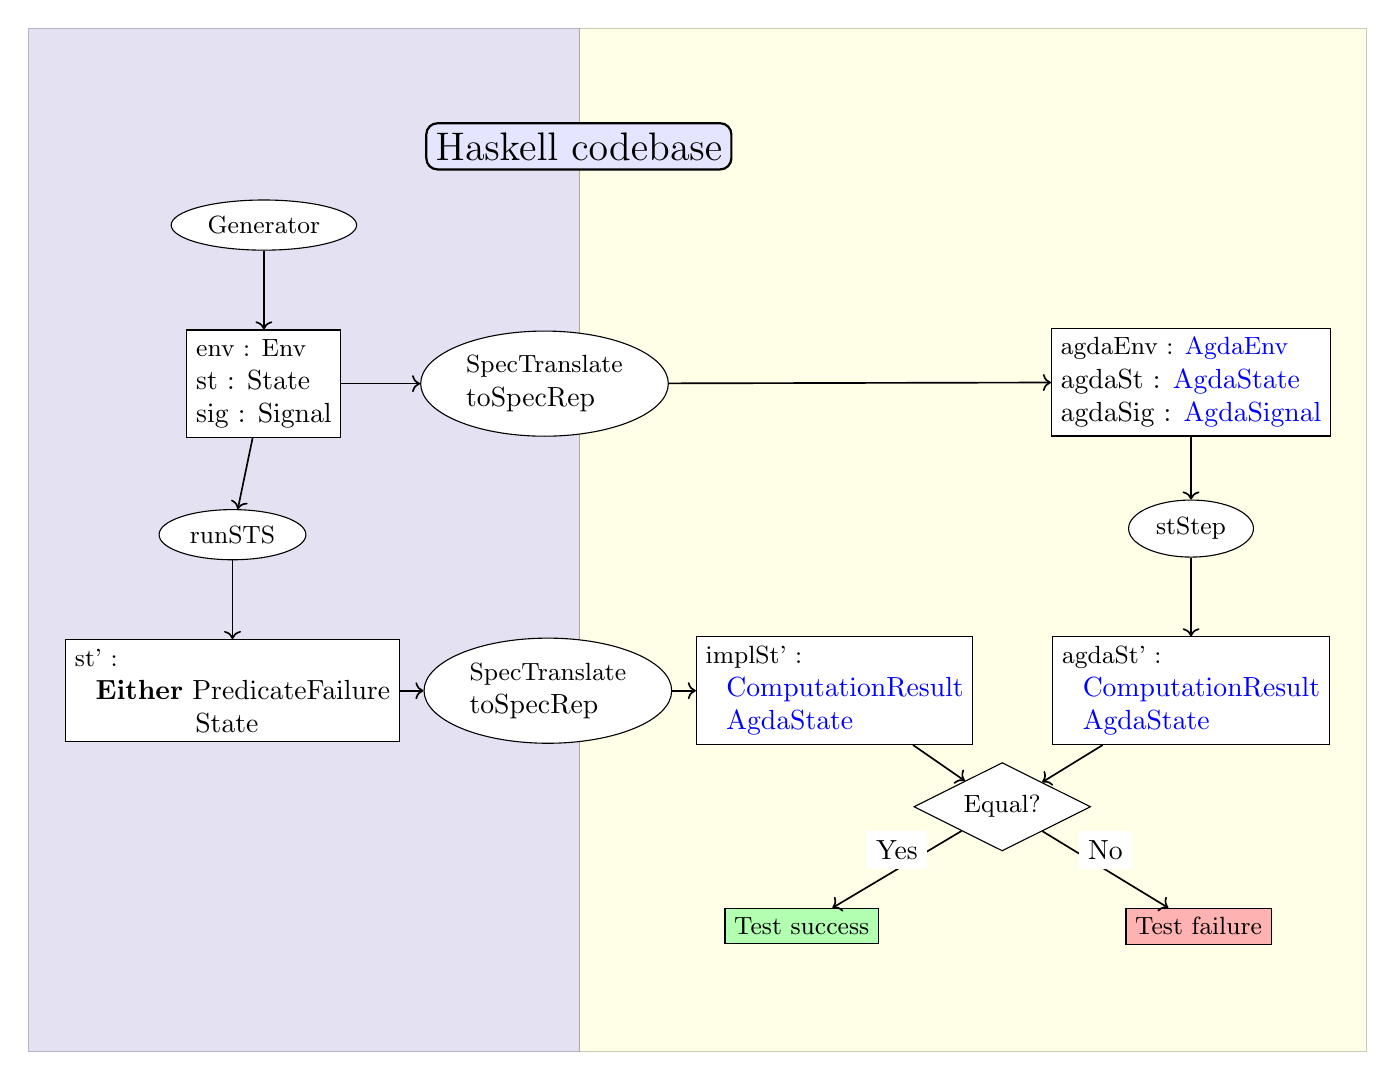
\begin{tikzpicture}[
    % node distance=10mm and 10mm,
    every node/.style={align=left, fill=white},
    rect/.style={draw, rectangle}, % -- , minimum height=10mm, minimum width=25mm},
    elpse/.style={draw, ellipse}, % , minimum height=10mm, minimum width=25mm},
    decision/.style={draw, diamond, aspect=2}, % , minimum height=10mm, minimum width=25mm},
    cloudstyle/.style={draw, rounded corners, thick, fill=blue!10}, % , text width=5cm, align=center},
%    note/.style={draw, cloud, cloud puffs=10, cloud puff arc=120, align=center, aspect=2},
    box/.style={draw, rectangle, fill=#1, inner sep=0pt, opacity=0.2, anchor=west, minimum height=13cm, minimum width=7cm},
    boxx/.style={draw, rectangle, fill=#1, inner sep=0pt, opacity=0.2, anchor=west, minimum height=13cm, minimum width=10cm},
    every edge/.style={draw, ->, >=Latex}
]

% Backgrounds
\node[box=\AlonzoColor] at (-7,0) {};
\node[boxx=\ConwayColor, anchor=west] at (0,0) {};

% Left section nodes
\node[elpse] (generator) at (-4, 4) {\small Generator};
\node[rect, below = of generator] (env) {\small env : Env\\ st : State\\ sig : Signal};
\node[elpse, below left=1cm and -1.25cm of env] (runSTS) {\small runSTS};
\node[rect, below =of runSTS] (stPrime) {\small st' :\\ \phantom{X}\textbf{Either} PredicateFailure\\\phantom{XxEither} State};

% Translation nodes
\node[elpse, right=1cm of env] (specTranslate1) {\small SpecTranslate\\ toSpecRep};
\node[elpse, right=3mm of stPrime] (specTranslate2) {\small SpecTranslate\\ toSpecRep};

% Right section nodes
% \node[rect] (blueNote) at (5.5, 4.5){\small Blue types and values are imported from\\ Malonzo modules which are compiled\\ directly from the Agda code};
\node[rect, right=3mm of specTranslate2] (implStPrime) {\small implSt' :\\ \phantom{X}\textcolor{blue}{ComputationResult}\\ \phantom{X}\textcolor{blue}{AgdaState}};
\node[rect, right=of implStPrime] (agdaStPrime) {\small agdaSt' :\\ \phantom{X}\textcolor{blue}{ComputationResult}\\ \phantom{X}\textcolor{blue}{AgdaState}};
\node[elpse, above=of agdaStPrime] (stStep) {\small stStep};
\node[rect, above=8mm of stStep] (agdaEnv) {\small agdaEnv : \textcolor{blue}{AgdaEnv}\\ agdaSt : \textcolor{blue}{AgdaState}\\ agdaSig : \textcolor{blue}{AgdaSignal}};

% Decision and results
\node[decision, below right=5mm and -2mm of implStPrime] (equal) {\small Equal?};
\node[rect, fill=red!30, below right=of equal] (testFail) {\small Test failure};
\node[rect, fill=green!30, below left=of equal] (testSuccess) {\small Test success};

% Left section edges
\draw[->,semithick] (generator) -- (env);
\draw[->,semithick] (env) -- (runSTS);
\draw[->,semithick] (runSTS) -- (stPrime);
\draw[->,semithick] (env) -- (specTranslate1);
\draw[->,semithick] (stPrime) -- (specTranslate2);

% Translation edges
\draw[->,semithick] (specTranslate1) -- (agdaEnv);
\draw[->,semithick] (specTranslate2) -- (implStPrime);

% Right section edges
\draw[->,semithick] (agdaEnv) -- (stStep);
\draw[->,semithick] (stStep) -- (agdaStPrime);
\draw[->,semithick] (agdaStPrime) -- (equal);
\draw[->,semithick] (implStPrime) -- (equal);

% Decision edges
\draw[->,semithick] (equal) -- node[above] {No} (testFail);
\draw[->,semithick] (equal) -- node[above] {Yes} (testSuccess);

% Labels
\node[cloudstyle] (haskellCodebaseLabel) at (0,5) {\Large Haskell codebase};
%[above right= of generator, font=\large\bfseries, fill=blue!10]
\end{tikzpicture}
\caption{Ledger conformance infrastructure; Blue types and values are imported from Malonzo modules which are compiled directly from the Agda code.}
\label{fig:conformance-infrastructure}
\end{figure}




\end{document}
